\lecture{4}{22.04.2021}{}
\begin{proof}
	\begin{enumerate}
		\item An easy consequence of the fact that $\subseteq$ on sets is reflexive and transitive.
		\item Assume that $C \sqsubseteq_{\mathcal{T}} D$.
			To show that $\forall r.C \sqsubseteq_{\mathcal{T}} \forall r.D$, we consider a model $\mathcal{I}$ of $\mathcal{T}$.
			We must show $ \left( \forall r.C \right)^{\mathcal{I}} \subseteq \left( \forall r.D \right)^{\mathcal{I}}$.
			Thus, let $d \in \left( \forall r.C \right)^{\mathcal{I}}$, i.e., for all $e \in \Delta^{\mathcal{I}}$,
			$\left( d,e \right) \in r^{\mathcal{I}} \implies e \in C^{\mathcal{I}}$.
			But then $C \sqsubseteq_{\mathcal{T}} D$ implies $C^{\mathcal{I}} \subseteq D^{\mathcal{I}}$.
			This yields $e \in D^{\mathcal{I}}$.
			Thus, $d \in \left( \forall r.C \right)^{\mathcal{I}}$.
			The proof for the existential restrictions is similar.
		\item Assume that $C \sqsubseteq_{\mathcal{T}} D$.
			Then, we have $C^{\mathcal{I}} \subseteq D^{\mathcal{I}}$ for all models $\mathcal{I}$ of $\mathcal{T}$.
			Let $\mathcal{T}'$ be such that $\mathcal{T} \subseteq \mathcal{T}'$.
			Then every model of $\mathcal{T}'$ is a model of $\mathcal{T}$.
			Thus, if $\mathcal{I}$ is a model of $\mathcal{T}'$, then $\mathcal{I}$ is a model of $\mathcal{T}$,
			and thus satisfies $C^{\mathcal{I}} \subseteq D^{\mathcal{I}}$.
			\qedhere
	\end{enumerate}
\end{proof}

\begin{lemma}
	Here are some basic equivalences:
	\begin{itemize}
		\item $\neg \top \equiv \bot$
		\item $C \sqcup D \equiv \neg \left( \neg C \sqcap \neg D \right)$
		\item $\forall r.C \equiv \neg \exists r.\neg C$
		\item $\exists r.\bot \equiv \bot$
		\item $\neg \left( \geq nr.C \right) \equiv \left( \leq n-1 r.C \right)$ if $n \geq 1$
		\item $\left( \geq 0 r.C \right) \equiv \top$
		\item $\left( \leq 0r.C \right) \equiv \forall r.\neg C$
	 \end{itemize}
\end{lemma}
\begin{proof}
	Lets have a closer look at $\forall r.C \equiv \neg \exists r.\neg C $.
	Let $\mathcal{I}$ be an interpretation.
	\begin{align*}
		d \in \left( \forall r.C \right)^{\mathcal{I}} & \iff \text{for all $e$ with $(d,e)\in r^{\mathcal{I}}$ we have $e \in C^{\mathcal{I}}$} \\
							& \iff \text{there is no $e$ with $(d,e)\in r^{\mathcal{I}}$ and $e \notin C^{\mathcal{I}}$} \\
							& \iff d  \notin \left( \exists r.\neg C \right)^{\mathcal{I}} \\
							& \iff d \in \left( \neg \exists r.(\neg C) \right)^{\mathcal{I}}
	\end{align*}
	Similar for the other equivalences. \qedhere
\end{proof}

\begin{definition}[assertional reasoning]
	Let $\mathcal{K} = \left( \mathcal{T}, \mathcal{A} \right)$ be a knowledge base, 
	$C$ a concept description and $a \in \mathscr{I}$.
	We then consider the following decision problems:
	\begin{enumerate}
		\item Knowledge base consistency: $\mathcal{K}$ is consistent iff there exists a model of $\mathcal{K}$.
		\item Instance: $a$ is an instance of $C$ w.r.t.\ $\mathcal{K}$ iff $a^{\mathcal{I}} \in C^{\mathcal{I}}$ 
			for all models $\mathcal{I}$ of $\mathcal{K}$.
	\end{enumerate}
\end{definition}
\begin{lemma}
	Let $\mathcal{K} = \left( \mathcal{T}, \mathcal{A} \right)$ be a knowledge base.
	If $a$ is an instance of $C$ w.r.t.\ $\mathcal{K}$ and $C \sqsubseteq_{\mathcal{T}} D$,
	then $a$ is an instance of $D$ w.r.t.\ $\mathcal{K}$.
\end{lemma}
\begin{proof}
	To Do !
\end{proof}

In the following we will show, that there exist certain polynomial reductions between the decision problems shown before:
\begin{figure}[H]
	\centering
	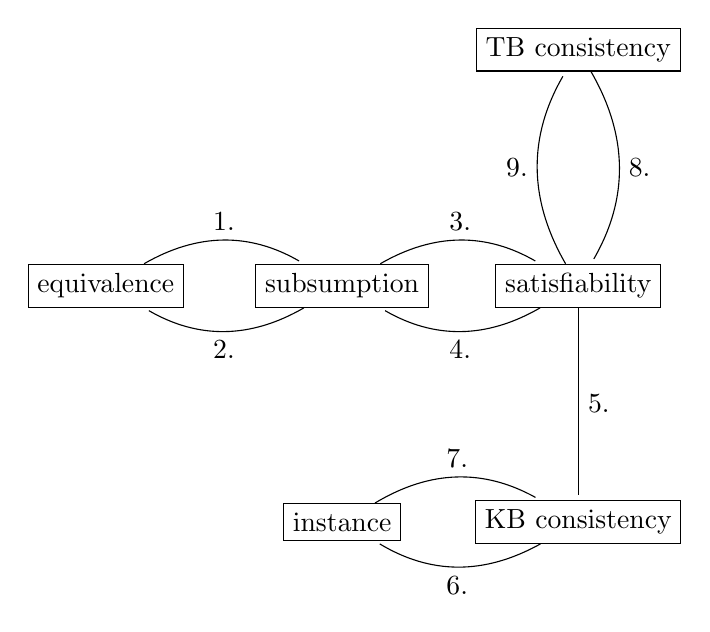
\begin{tikzpicture}[align=center,node distance=3cm, shorten >= 2pt]
		\node[draw] (eq) {equivalence};
		\node[draw, right of = eq] (sub) {subsumption};
		\node[draw, right of = sub] (sat) {satisfiability};
		\node[draw, below of = sat] (kbc) {KB consistency};
		\node[draw, left of = kbc] (ins) {instance};
		\node[draw, above of = sat] (tbc) {TB consistency};
		\draw (eq) edge[above, bend left] node{1.} (sub);
		\draw (sub) edge[below, bend left] node{2.} (eq);
		\draw (sub) edge[above, bend left] node{3.} (sat);
		\draw (sat) edge[below, bend left] node{4.} (sub);
		\draw (sat) edge[right]  node{5.} (kbc);
		\draw (kbc) edge[below, bend left] node{6.} (ins);
		\draw (ins) edge[above, bend left] node{7.} (kbc);
		\draw (tbc) edge[right, bend left] node{8.} (sat);
		\draw (sat) edge[left, bend left] node{9.} (tbc);
	\end{tikzpicture}
	\caption{Polynomial reductions between decision problems.}
	\label{fig:problem reductions}
\end{figure}
\begin{note}
	These reductions do not only hold for $\mathcal{ALC}$, but for all DLs with the constructors negation and conjunction.
	The last one also needs an existential quantifier.
	They correspond to the following lemma:
\end{note}

\begin{theorem}
	Let $\mathcal{K} = \left( \mathcal{T}, \mathcal{A} \right)$ be a knowledge base, 
	$C, D$ concept descriptions and $a \in \mathscr{I}$.
	\begin{enumerate}
		\item $C \equiv_{\mathcal{T}} D \iff C \sqsubseteq_{\mathcal{T}} D \land D \sqsubseteq_{\mathcal{T}} C$ 
		\item $C \sqsubseteq_{\mathcal{T}} D \iff C \equiv_{\mathcal{T}} C \sqcap D$
		\item $C \sqsubseteq_{\mathcal{T}} D \iff C \sqcap \neg D$ is unsatisfiable w.r.t.\ $\mathcal{T}$
		\item $C$ is satisfiable w.r.t.\ $\mathcal{T} \iff C \not\sqsubseteq_{\mathcal{T}} \bot$
		\item $C$ is satisfiable w.r.t.\ $\mathcal{T} \iff \left( \mathcal{T}, \left\{ a:C \right\} \right)$ is consistent
		\item $a$ is an instance of $C$ w.r.t.\ $\mathcal{K} \iff \left( \mathcal{T}, \mathcal{A} \cup \left\{ a: \neg C \right\} \right)$ is inconsistent
		\item $\mathcal{K}$ is consistent $\iff a$ is not an instance of $\bot$ w.r.t.\ $\mathcal{K}$
		\item $\mathcal{T}$ is consistent $\iff \top$ is satisfiable w.r.t.\ $\mathcal{T}$
		\item $C$ is satisfiable w.r.t.\ $\mathcal{T} \iff \mathcal{T} \cup \left\{ \top \sqsubseteq \exists r.C \right\}$,
			where $r$ is a new role that does not occur in $C$ or $\mathcal{T}$,
			is consistent.
	\end{enumerate}
\end{theorem}
\begin{proof}
	\begin{enumerate}
		\item By definition.
		\item An easy consequence of the set inclusion relation $\subseteq$.
		\item
			\begin{align*}
				C \sqsubseteq_{\mathcal{T}} D & \iff \forall \mathcal{I}, \mathcal{I} \vDash \mathcal{T}: C^{\mathcal{I}} \subseteq D^{\mathcal{I}}\\
											  & \iff \forall \mathcal{I}, \mathcal{I} \vDash \mathcal{T} : C^\mathcal{I} \cap (\Delta^{\mathcal{I}} \setminus D^{\mathcal{I}}) = \emptyset\\
											  & \iff \forall \mathcal{I}, \mathcal{I} \vDash \mathcal{T}: C^{\mathcal{I}} \cap (\neg D)^\mathcal{I} = \emptyset\\
											  & \iff \forall \mathcal{I}, \mathcal{I} \vDash \mathcal{T}: \left( C \sqcap \neg D \right)^\mathcal{I} = \emptyset\\
											  & \iff \left( C \sqcap \neg D \right) \text{is unsatisfiable w.r.t.}\ \mathcal{T} 
			\end{align*}
		\item trivial.
		\item see lecture video.
		\item "$ \implies$": By its contraposition. \newline
			Assume that $\left( \mathcal{T}, \mathcal{A} \cup \left\{a: \neg C \right\} \right)$ is indeed consistent.
			Then there is  a model $\mathcal{I}$ of $\mathcal{T} , \mathcal{A}$ and $\left\{ a: \neg C \right\}$.
			But then $\mathcal{I}$ is a model of $\mathcal{K} = \left( \mathcal{T}, \mathcal{A} \right)$ such that
			$a^{\mathcal{I}} \notin C^\mathcal{I}$.
			Thus, $a$ is not an instance of $C$ w.r.t.\ $\mathcal{K}$. \newline
			"$\impliedby$": Also by its contraposition. \newline
			Assume that $a$ in not an instance of $C$ w.r.t.\ $\mathcal{K}$.
			Thus there is a model $\mathcal{I}$ of $\mathcal{K}$ with $a^\mathcal{I} \notin C^\mathcal{I}$.
			Thus, $\mathcal{I}$ is a model of $\left( \mathcal{T}, \mathcal{A} \cup \left\{ a: \neg C \right\} \right)$.
		\item By the contraposition: \newline
			Assume that $\mathcal{K}$ is consistent and let $\mathcal{I}$ be a model of $\mathcal{K}$.
			Then $a^\mathcal{I} \notin \emptyset = \bot^\mathcal{I}$.
			If $\mathcal{K}$ is inconsistent, then there is no model of $\mathcal{K}$.
			Thus $a^{\mathcal{I}} \in \bot^\mathcal{I}$ holds in all models since there are none.
		\item see lecture video.
		\item "$ \implies$": \newline
			Assume that $\mathcal{I}$ is a model of $\mathcal{T}$ such that $C^\mathcal{I} \neq \emptyset$
			(definition of satisfiability).
			Let $d \in C^{\mathcal{I}}$.
			We extend $\mathcal{I}$ to $\mathcal{I}'$by setting $r^{\mathcal{I}} = \left\{ (e,d) \mid  e \in \Delta^{\mathcal{I}} \right\}$.
			Since $r$ does not occur in $C$ or $\mathcal{T}$, we still have $d \in C^\mathcal{I'}$ and $\mathcal{I'}$ is a model of $\mathcal{T}$. \newline
			"$\impliedby$": \newline
			If $\mathcal{I}$ is a model of $\mathcal{T} \cup \left\{ \top \sqsubseteq \exists r.C \right\}$,
			then let $e$ be an arbitrary element of $\Delta^{\mathcal{I}}$.
			Then $e \in \left( \exists r.C \right)^{\mathcal{I}}$, and thus there is an $d \in \Delta^{\mathcal{I}}$ 
			with $\left( e,d \right) \in r^{\mathcal{I}}$ and $d \in C^\mathcal{I}$.
			Thus, $C$ is satisfiable w.r.t.\ $\mathcal{T}$.
			\qedhere
	\end{enumerate}
\end{proof}

Now we will show, that satisfiability w.r.t.\ $\mathcal{T}$ can be reduced to satisfiability (without $\mathcal{T}$) and
Knowledge base consistency can be reduced to ABox consistency.
However this reduction is in general not possible in polynomial time.

\begin{prop}
Let  $\mathcal{K} = (\mathcal{T}, \mathcal{A})$ be a knowledge base, where $\mathcal{T}$ is acyclic, and $C$ a concept description.
The expanded versions $\widehat{C}$ and $\widehat{A}$ of $C$ and $A$ w.r.t.\ $\mathcal{T}$ are obtained by
replacing all defined concepts occurring in $C$ and $A$ by their definitions in the expanded version $\widehat{\mathcal{T}}$ of $\mathcal{T}$.
Then:
	\begin{enumerate}
		\item $C$ is satisfiable w.r.t.\ $\mathcal{T} \iff \widehat{C}$ is satisfiable.
		\item $\mathcal{K} = (\mathcal{T},\mathcal{A})$ is consistent $\iff (\emptyset,\widehat{\mathcal{A}}$) is consistent.
	\end{enumerate}
\end{prop}
\begin{merke}[frametitle=Important Note:]
	The problem of deciding whether $(\emptyset, \widehat{\mathcal{A}})$ is consistent is also called "ABox consistency".
	The proposition above shows, that each of the decision problems discussed before can be reduce to ABox consistency,
	as long as no cyclic TBox is involved.
\end{merke}
\begin{proof}
	\begin{enumerate}
		\item " $\implies$":\newline
			Let $\mathcal{I}$ be a model of $\mathcal{T}$ with $C^\mathcal{I} \neq \emptyset$.
			Then $\mathcal{I}$ is also a model of $\widehat{\mathcal{T}}$ and we have $\emptyset \neq C^\mathcal{I} = \widehat{C}^\mathcal{I}$.
			Thus, $\widehat{C}$ is satisfiable. \newline
			"$\impliedby$": \newline
			Let $\mathcal{I}$ be an interpretation with $\widehat{C}^{\mathcal{I}} \neq \emptyset$.
			Let $\mathcal{J}$ be the primitive interpretation of which $\mathcal{I}$ is an extension
			and let $\mathcal{I}'$ be the model of $\mathcal{T}$ that extends $\mathcal{J}$.
			Since $\widehat{C}$ contains only primitive concepts,
			we have $\emptyset \neq \widehat{C}^{\mathcal{I}} = \widehat{C}^\mathcal{J} = \widehat{C}^{\mathcal{I'}} = C^{\mathcal{I'}}$,
			since $\mathcal{I}'$ is a model of $\mathcal{T}$ and $\widehat{\mathcal{T}}$.
		\item similar
			\qedhere
	\end{enumerate}
\end{proof}
\newpage
